% Chapter Template

\chapter{Introduction} % Main chapter title

\label{Chapter1} % Change X to a consecutive number; for referencing this chapter elsewhere, use \ref{ChapterX}

%----------------------------------------------------------------------------------------
%	SECTION 1
%----------------------------------------------------------------------------------------
%
% Statment of the problem + Motivation
%
Quantum computing is a new paradigm of computation whose importance is growing not only by its promising speed-up over classical computers in some problems such as combinational optimization problems but also by the fact that we are building transistors in a scale where quantum effects are starting to appear. Combinational optimization problems are common among industry albeit more research need to be done to get insight about how quantum computing could help to solve industry challenges. There is already a large industry research in finances [\textbf{REFERENCIAS}], route planning [\textbf{REFERENCIAS}], cybersecurity [\textbf{REFERENCIAS}] and life science among others. From our point of view, there is a lack of published\footnote{Currently, there are private companies that are pursing research in this field such as E-ON\,\cite{Fernandez-Campoamor2021CommunityAnnealing}.} research in the energy sector, so we decided to contribute to that field.\\\\
\begin{figure}[H]
  \begin{center}
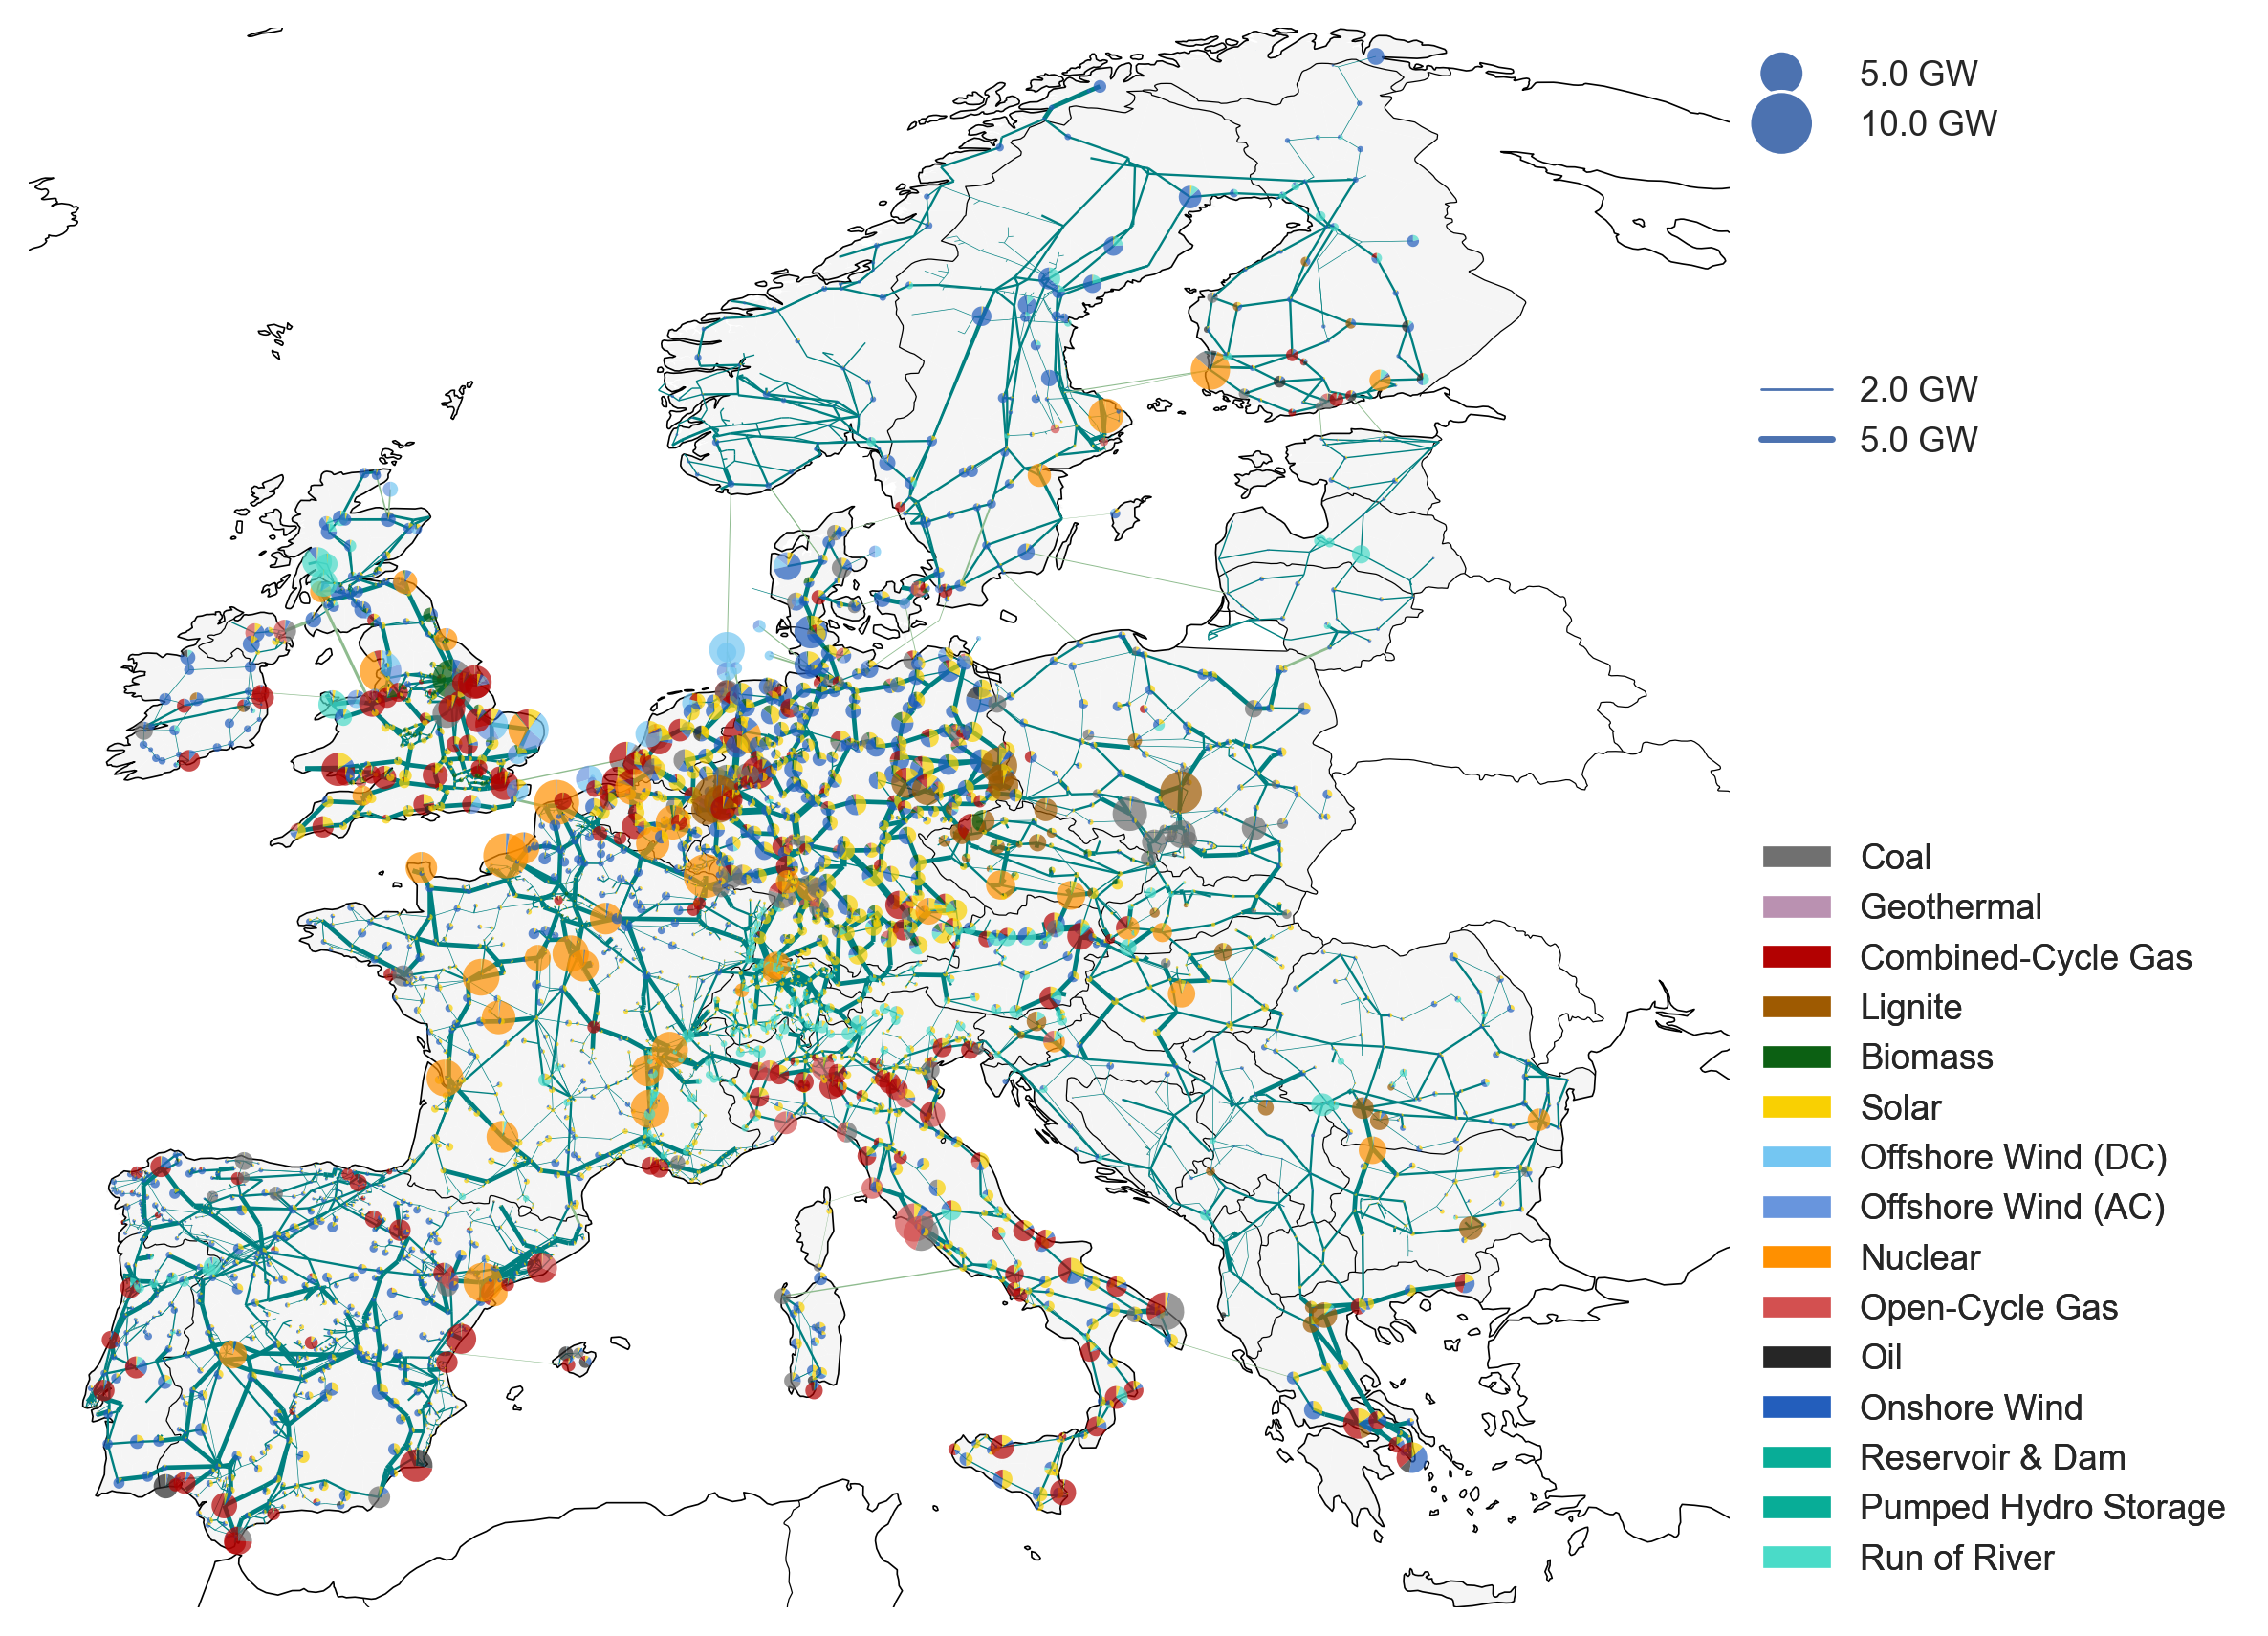
\includegraphics[width=0.9\textwidth]{Figures/Europe-Grid.png}
  \end{center}
  \caption{Clustered transmission network model of Europe.\textbf{Preguntar a Oriol}}
\end{figure}
Energy system models are getting larger and more complex due to the integration of decentralized weather-dependent renewable energy sources, intermittent loads, sector coupling and the increase of storage components. For instance, the renewable energy produced by the integration of solar panels in dwellings is though to be integrated to the grid if the consumers are not using it, but the grid infrastructure is not evolving accordingly to the new energy paradigm. As a consequence, energy from private sources cannot be added to the grid which implies the efficiency of solar panels has to be decreased or the excess of energy has to be dropped. A good infrastructure would solve this problems by addressing the excess of energy to where is required and by storing the excess so it can be used later, e.g., to charge an electric car in a fuel station. In this way the energy would be efficiently distributed and energy companies could offer better prices to their consumers while safeguarding the environment by reducing their carbon footprints. Furthermore an increment of the quantity of detailed data about energy consumption -- smart meters -- would extend the spatial and temporal resolution, i.e., the grid status of a region, so that better managing and expansion planning decisions can be made in order to satisfy the customer demand efficiently.\\\\ 
The problem we tackled in the present work is called transmission expansion problem (TEP) which is a \textit{mixed integer linear problem} (MILP), with NP complexity, i.e., an increment in the spatial and time resolution entails an exponential grow in the number of variables for the MILP making the problem intractable for a classical computer. Currently, the scope and granularity of the model are reduced using clustering algorithms. For this reason, any computational time reduction will have substantial implications in closing the granularity gap between what the current models can solve and the desired resolution needed by energy system operators.\\\\
Quantum computers are the candidates to solve NP-hard problems such as MILP, by making the complexity of the problem scale polemically as the systems size grows. Concretely, quantum analog computers are single-purpose quantum computers specialised in solving combinational optimization problems. The size of analog computers, i.e., the number of qubits of the system is greater than the general purpose quantum computers -- digital computers -- such as the ones from IBM that are based in the successive applications of quantum gates, e.g., Osprey with 433 qubits.
%
% Objectives of my thesis
%
Although quantum computers are getting bigger every few years they are not mature enough for solving many real-world problems where the number of variables scale exponentially. Also, we have to take into account that quantum computers are hugely affected by the environment conditions -- Intermediate-Scale Quantum (NISQ) era --, so there are errors during a code execution and the execution time has to be short enough so that it does not exceed quantum decoherence. The current maturity of quantum computers required of an hybrid quantum-classical approach to tackle real-world problems. The hybrid approach combine classical solvers and cutting-edge classical algorithms with quantum solvers that add the speed-up where it is possible.\\\\
A benchmark of how a TEP problem can be scaled until a quantum solver is not able to find a solution is provided among with a scheme to decompose a large TEP problem into a small enough master problem that can be addressed by a quantum computer and a sub-problem addressed by a classical computer. \\\\
% Structure of the thesis
%
The present work is structured as follows. Chapter\,\ref{Chapter2} guides through the foundations of adiabatic quantum computing. Chapter\,\ref{Chapter3} describes Benders' decomposition techniques. Chapter\,\ref{Chapter4} solve a transmission expansion problem by starting with a small network solved by a pure quantum annealer and ending up with a bigger network that requires from hybrid solvers. Conclusions and outlook are drawn in Chapter\,\ref{Chapter5}.
